\part{Introducción}
\pagenumbering{arabic}

\chapter{Introducción y visión general}


En este capítulo se hará una breve introducción para entender el contexto de este trabajo y el porqué de la necesidad del mismo. Se comentará la importancia de la localización para los seres humanos y se hará una introducción sobre los mapas utilizados por los robots para localizarse. Finalmente se expondrá la estructura del documento.\\

\section{La localización como una necesidad}

Que levante la mano quien no se ha perdido alguna vez por los despachos de alguna de las facultades, sobre todo en esos ambientes prácticamente idénticos entre sí. Todo ser humano alguna vez se ha parado en seco, ha mirado a un lado y a otro con cara de desaprobación y se ha preguntado: \textit{¿dónde estoy?} Estas situaciones, a veces incómodas, se deben esencialmente a que todo ser vivo con capacidad para desplazarse por un entorno necesita localizarse y orientarse si quiere alcanzar un objetivo, más aún si dicho entorno es totalmente desconocido.\\

A lo largo de los años, los seres humanos hemos utilizado multitud de métodos para la orientación, incluso en las situaciones más desfavorables. Un estudio para la revista \textit{The Royal Society} de la Universidad de Rennes sostiene que los vikingos usaban una variedad de calcita para calcular dónde se encontraba el sol utilizando la polarización de la luz dispersada por las nubes. Esta piedra solar se llama ``Espato de Islandia'' y les permitía orientarse incluso en fechas donde el sol parecía no querer mostrarse, algo que sucede muy frecuentemente en los mares nórdicos \cite{vikingos}. Hoy en día, con el uso de la tecnología GPS y de aplicaciones que la implementan como Google Maps, hemos cambiado esa piedra solar por un dispositivo electrónico que, no solo nos localiza y orienta en prácticamente cualquier situación, sino que lo hace con un error casi despreciable. Pese al avance de las tecnología de localización como GPS, existen ciertas situaciones en las que es complicado aprovecharse de ellas, como por ejemplo en los entornos indoor. En estos caso, los satélites no son capaces de comunicarse con nuestros dispositivos, por lo que necesitamos de otro mecanismo para localizarnos.\\

%\begin{figure}[H]
%	\begin{center} 
%	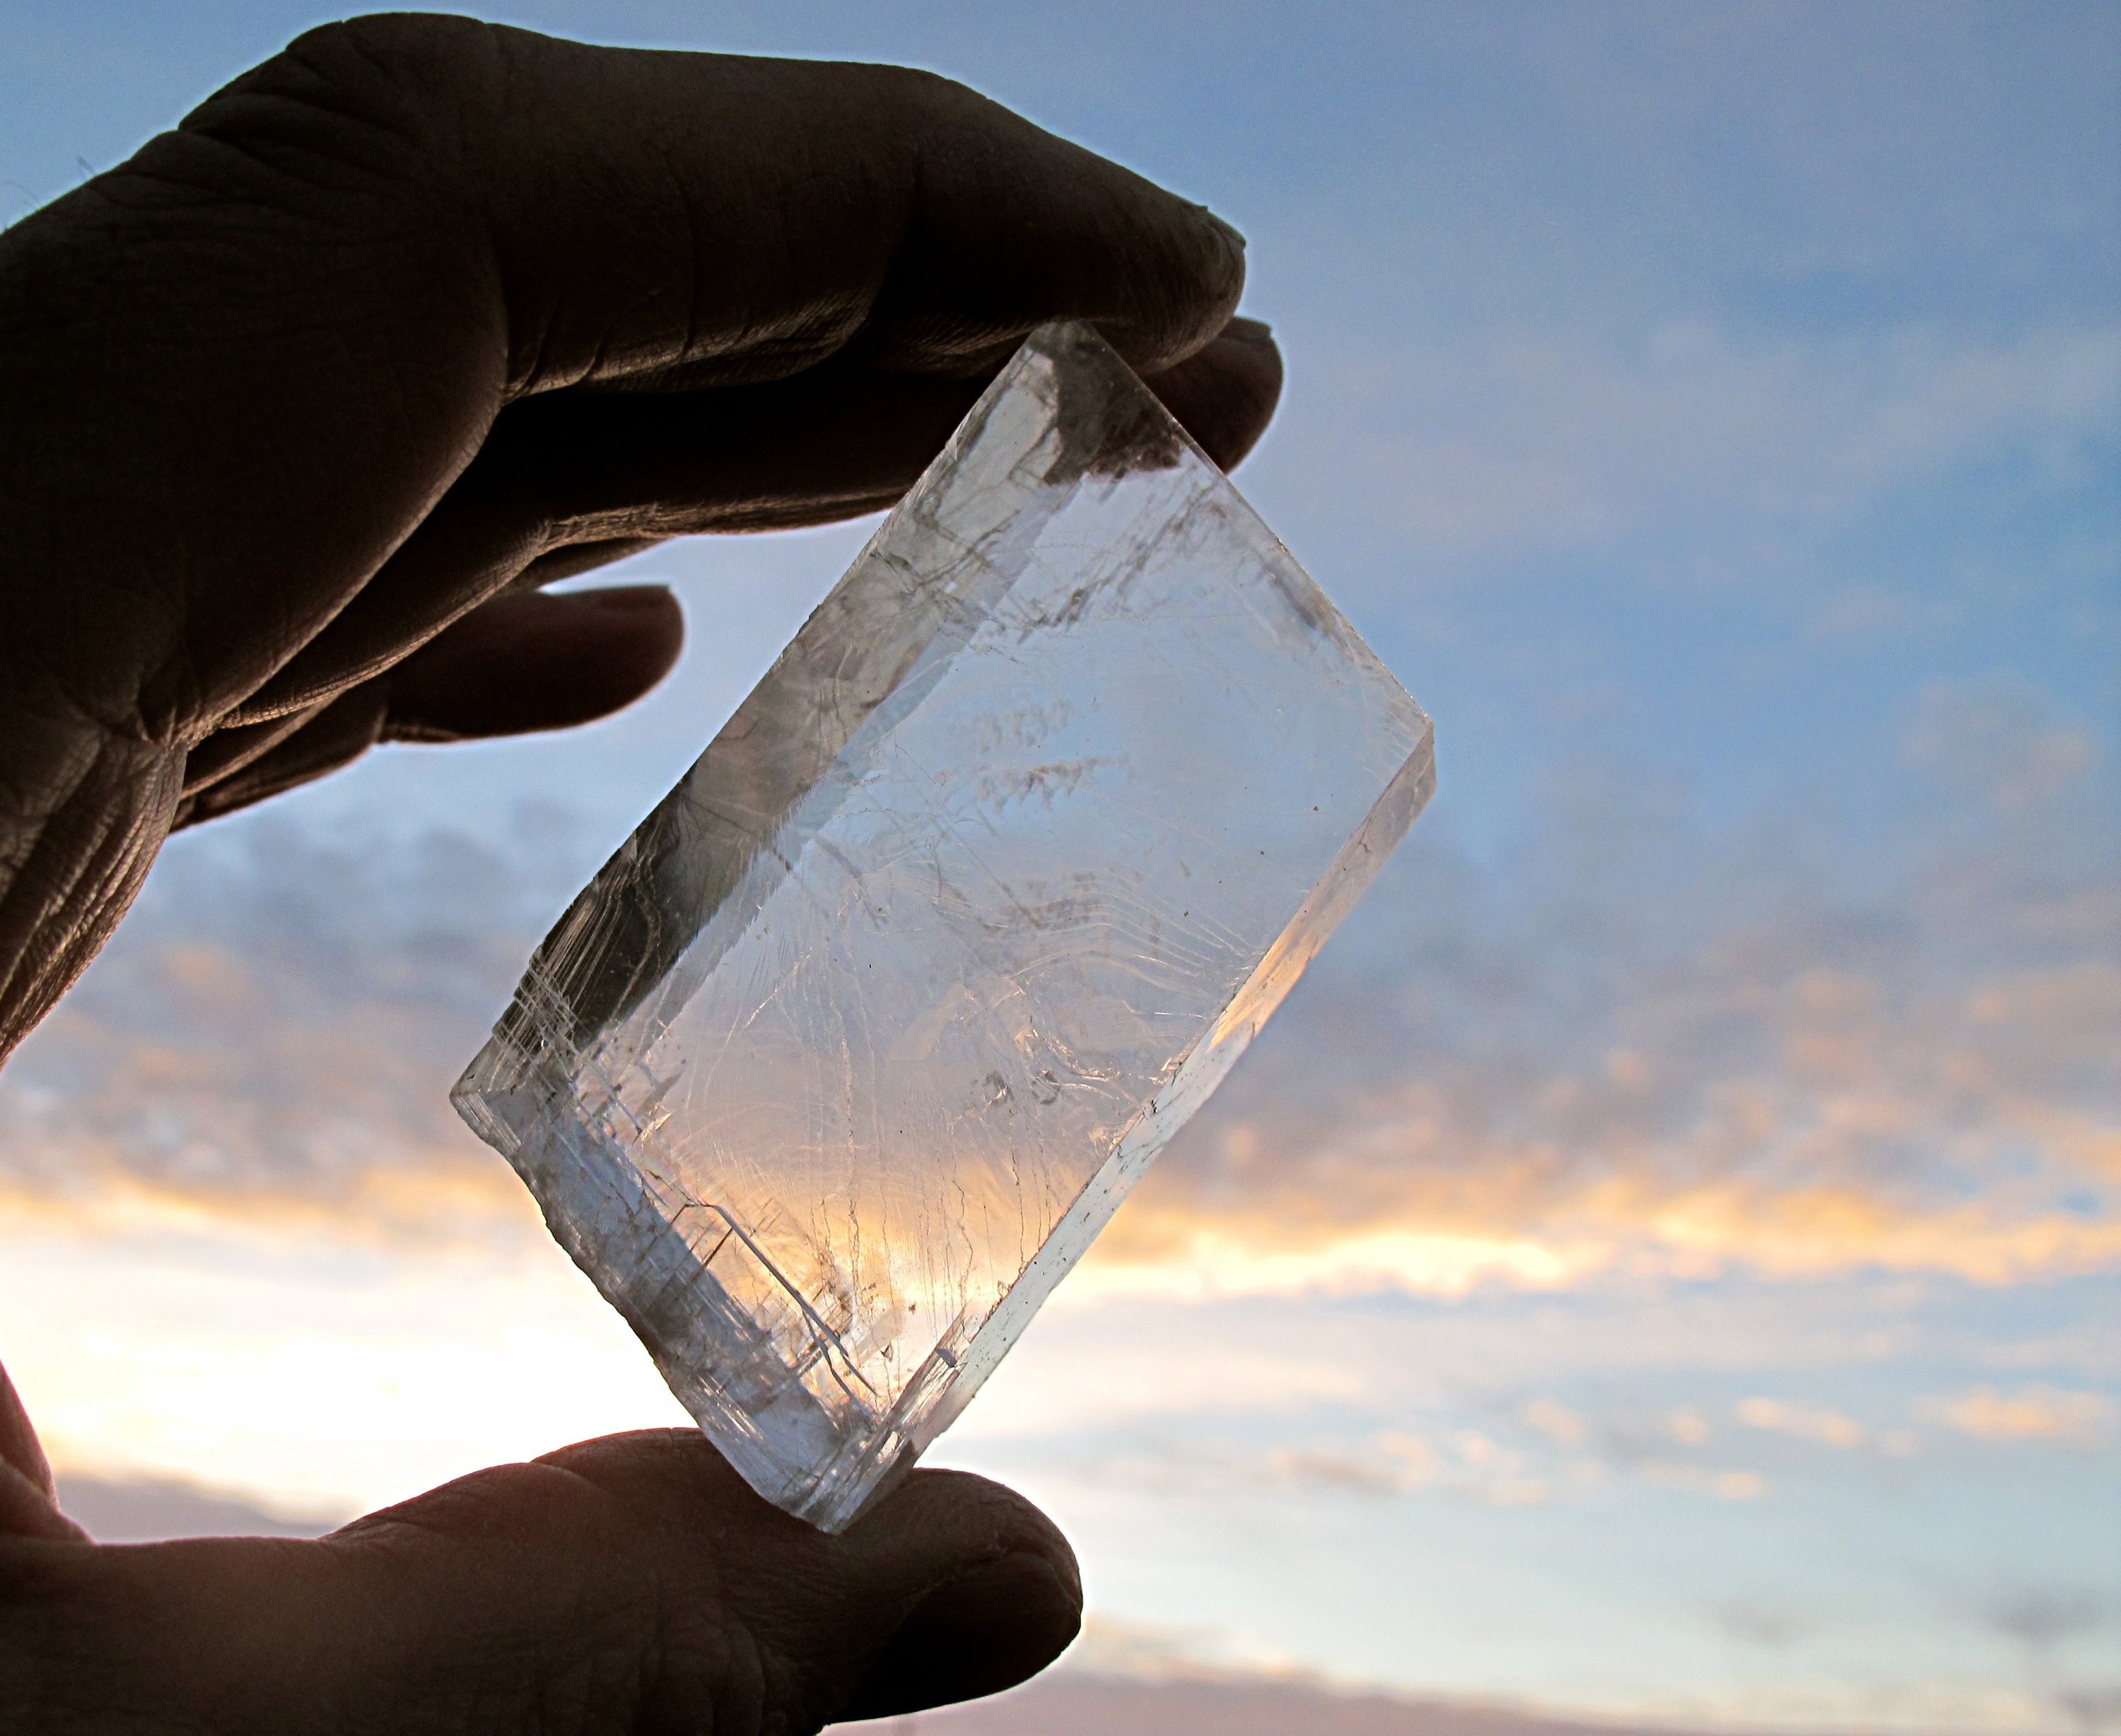
\includegraphics[width=0.5\textwidth]{espato_islandia.jpg}
%	\end{center}
%	\caption{Espato de Islandia. Variedad de piedra caliza \cite{espato}}
%	\label{fig:espato}
%\end{figure}

En la figura \ref{fig:metro} se muestra una parte del plano de la red de metro de la Comunidad de Madrid. A primera vista, uno se pierde entre tanto entresijo de líneas de colores pero si se establece una estación de origen y otra de destino, este plano facilita, e incluso posibilita, concretar el camino a tomar. Además, en las estaciones suele haber una gran cantidad de señalizaciones que hacen aún más fácil la localización. Entonces, si los humanos, seres inteligentes con percepción visual y capacidad de razonamiento, necesitamos localizarnos para alcanzar un objetivo, ¿porqué no lo iban a necesitar los robots? \\

\begin{figure}[h]
	\begin{center} 
	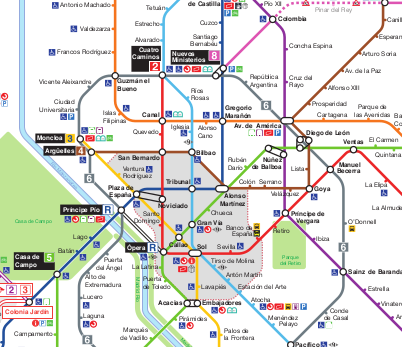
\includegraphics[width=0.4\textwidth]{plano_metro.png}
	\end{center}
	\caption{Detalle de la red de metro de la Comunidad de Madrid. \cite{metro_madrid}}
	\label{fig:metro}
\end{figure}

%\begin{figure}[H]
% \centering
%  \subfloat[Coeficiente $K=0$]{
%    \includegraphics[width=0.3\textwidth]{p6/simk0_ej1.png}}
%  \subfloat[Coeficiente $K=1$]{
%    \includegraphics[width=0.3\textwidth]{p6/simk1_ej1.png}}
% \caption{Simulación de la posición cartesiana para diferentes valores de %$K$}
% \label{fig:p6:sim_ej1}
%\end{figure}

La robótica móvil ha ido evolucionando a un ritmo vertiginoso desde que comenzó a desarrollarse. En los años sesenta se diseñó el apodado como \textit{SHAKEY} o ``el primer robot inteligente móvil del mundo'' según el IEEE (Instituto de Ingenieros Eléctricos y Electrónicos, del inglés \textit{Institute of Electrical and Electronics Engineers}). Este robot era el primero de su generación capaz de navegar en un entorno no controlado, sirviéndose de múltiples dispositivos que le proporcionaban información sobre la distribución de los elementos que le rodeaban, dándole la posibilidad al robot de evitarlos durante el trayecto \cite{shakey1}.\\

\begin{figure}[h]
	\begin{center} 
	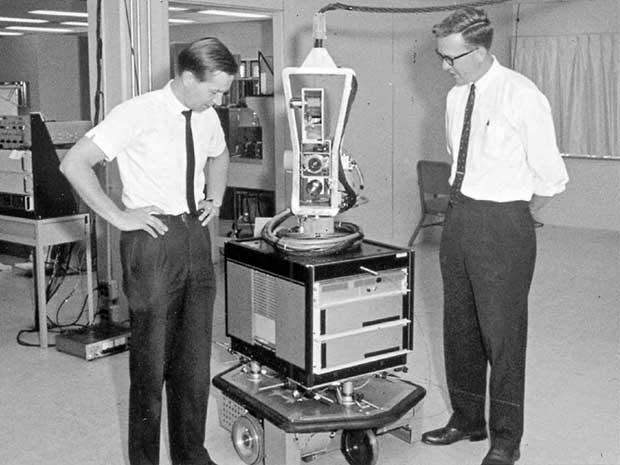
\includegraphics[width=0.8\textwidth]{shakey.jpg}
	\end{center}
	\caption{Foto tomada del robot SHAKEY en 1968. \cite{shakey2}}
	\label{fig:shakey}
\end{figure}


Un robot autónomo móvil (ARM) es un robot capaz de navegar a través de un entorno sin supervisión directa por parte de un operador humano ni la necesidad de disponer de un ruta fijada previamente. Para poder llevarlo a cabo, los robots disponen de multitud de sensores que les permiten percibir e interpretar el entorno, dotando al robot de la capacidad de navegar por el mismo evitando obstáculos, tanto fijos como móviles. Para poder realizar una navegación de alto nivel que les permita ir desde un punto origen a otro punto destino, los robots se sirven de mapas. Un mapa es una representación bidimensional del entorno. Existen dos tipos de mapas de aplicación a la robótica: los mapas métricos y los mapas topológicos. Los mapas métricos (figura \ref{fig:mapas}, izquierda) dividen el entorno en una rejilla donde cada celda representa una probabilidad de estar ocupada o de no estarlo. Si se discretiza esa probabilidad el resultado es un mapa de ocupación, (también llamado \textit{floorplan} o ``plano de suelo'', en un ámbito menos técnico), si no, se obtiene un mapa probabilístico. El mapa métrico más simple es el formado por un conjunto de referencias visuales o \textit{landmarks} de posición conocida que ayudan al robot a estimar su posición. Los mapas topológicos (figura \ref{fig:mapas}, derecha) están basados en grafos y representan la conectividad entre cada uno de sus nodos. Existe una tercer tipo de mapa que es un híbrido entre los comentados y es el más utilizado para los robots: utilizan los grafos para la generación de trayectorias (navegación) y el mapa métrico para la localización.\\

\begin{figure}[H]
 \centering
  \subfloat[Ejemplo de mapa métrico: mapa de ocupación]{
    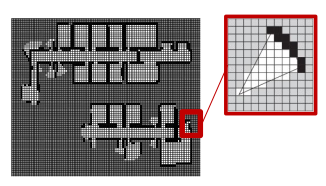
\includegraphics[width=0.35\textwidth]{mapa_ocupacion.png}}
  \hspace{2cm}
  \subfloat[Mapa topológico: líneas del metro de Málaga \cite{metro_malaga}]{
    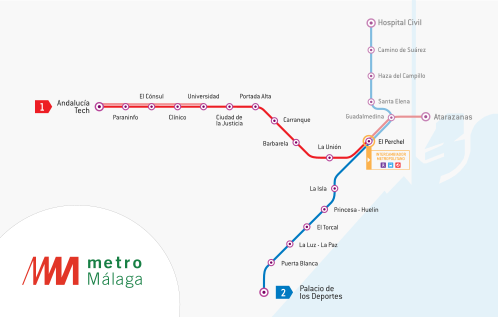
\includegraphics[width=0.3\textwidth]{metro_malaga.png}}
 \caption{Ejemplos de tipos de mapas.}
 \label{fig:mapas}
\end{figure}

Los mapas métricos más utilizados en la robótica móvil son los mapas de ocupación o \textit{floorplans}. Son generados en una primera fase de inspección del entorno, empleando los mismos sensores que luego servirán para la navegación autónoma. Tradicionalmente, estos mapas de ocupación son generados empleando un láser 2D o LIDAR (dado su gran alcance y amplio campo de visión), generando por tanto mapas bidimensionales que especifican aquellas zonas del entorno que están libres de obstáculos y por tanto susceptibles de navegación, y aquellas que no lo están. No obstante, dado que un láser 2D no puede distinguir entre los objetos detectados, los mapas de ocupación bidimensionales generados con este sensor contienen, no sólo los elementos estructurales del entorno como paredes, puertas, columnas, etc., si no que incluyen multitud de objetos como mesas y sillas, camas, cajas e incluso personas si estaban presentes en el momento de generar el mapa.\\

La inclusión de estos elementos no estructurales en el mapa de ocupación puede ocasionar problemas si se pretende utilizar ese mapa durante un largo período de tiempo. El mapa generado no estaría preparado si el entorno que representa sufre algún tipo de modificación de mobiliario, por lo que sería necesario volver a generar un nuevo mapa, con todo lo que eso conlleva. Sin ir más lejos, en la Escuela de Ingenierías Industriales hay muchos elementos que no pertenecen a la estructura del edificio que, si hoy mismo se utilizara un robot equipado con un láser 2D para generar un mapa, ocasionarían los problemas ya comentados. Estos elementos son, por ejemplo, las impresoras que hay en algunas zonas, las máquinas de refrescos y snacks, papeleras, carteles publicitarios, las nuevas mesas instaladas en la zona central, etc (figura \ref{fig:laser_vs_rgbd}).\\

En la figura \ref{fig:errores_laser} se muestra un ejemplo de un mapa generado de un entorno virtual a través de un láser 2D de 360º. Como se puede observar hay zonas, marcadas con numeración, en las que el mapa no representa fielmente las dimensiones reales de la vivienda. De modo que, si los objetos que no forman parte de la estructura modifican su posición después de la primera fase de análisis, el mapa de ocupación generado no podría ser utilizado por el robot para la navegación. \\

\begin{figure}[h]
	\begin{center} 
	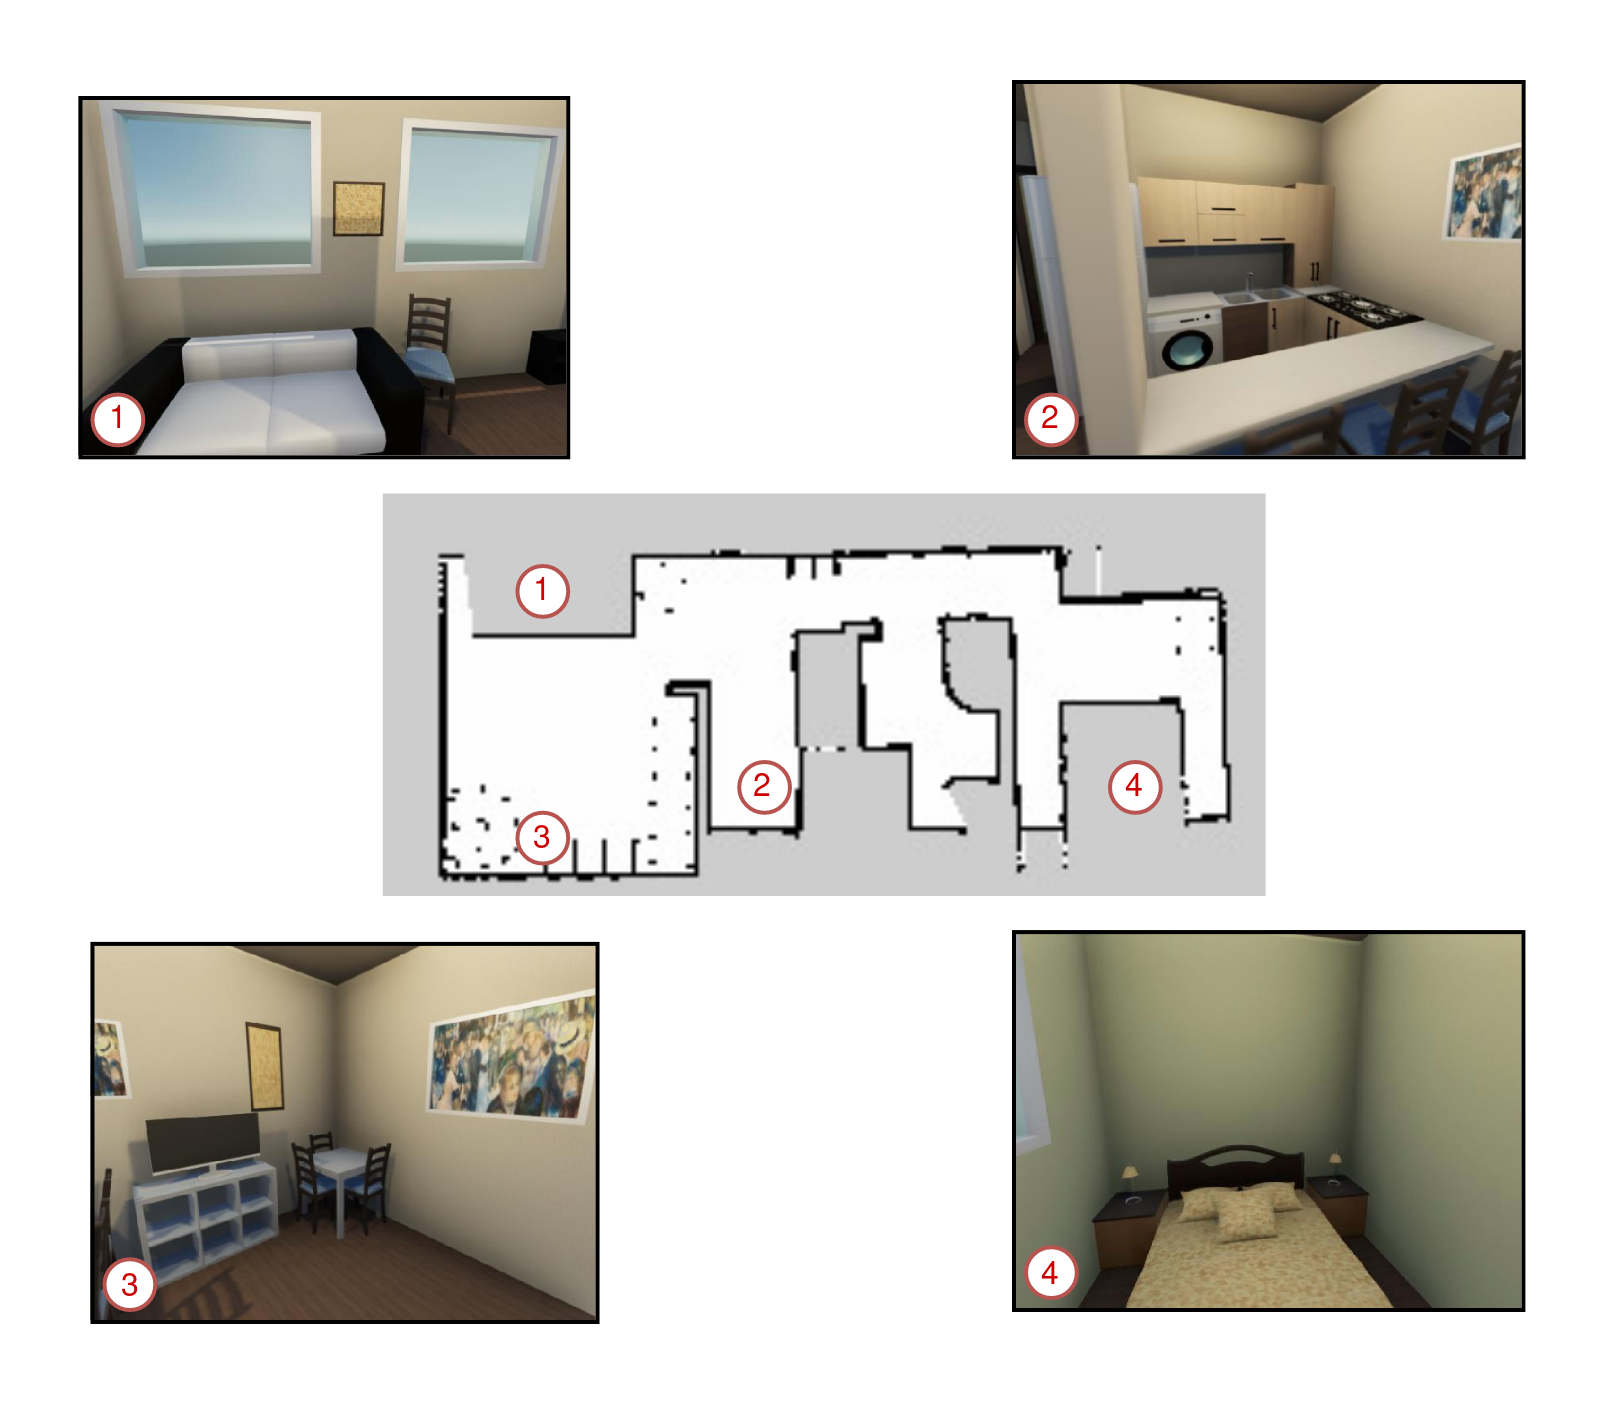
\includegraphics[width=0.8\textwidth]{IlustracionErroresMapa.png}
	\end{center}
	\caption{Mapa generado con el barrido de un láser. Las zonas enumeradas muestran que el mapa generado no representa fielmente la estructura del entorno debido a la presencia de elementos que pueden variar en su posición como un sofá, una silla, una cama, etc.}
	\label{fig:errores_laser}
\end{figure}

Dado que estos métodos de generación de mapas de ocupación mediante láser 2D sufren frente a la variabilidad en la distribución, surge la idea de utilizar otros sensores que permitan discernir entre los distintos elementos que pudieran formar parte del entorno. Los sensores RGBD son cámaras que, además de proporcionar información sobre el color, ofrecen la distancia a la que se encuentra cada píxel captado en la imagen con respecto a la cámara. Por lo tanto, ofrecen información en 3D del dominio, lo que abre más posibilidades a la hora de percibir e interpretar la información captada mediante los sensores. En la figura \ref{fig:laser_vs_rgbd} se muestra un ejemplo de lo que se quiere conseguir aprovechando las ventajas de los sensores RGBD frente a los láseres 2D.\\

\begin{figure}[H]
	\begin{center} 
	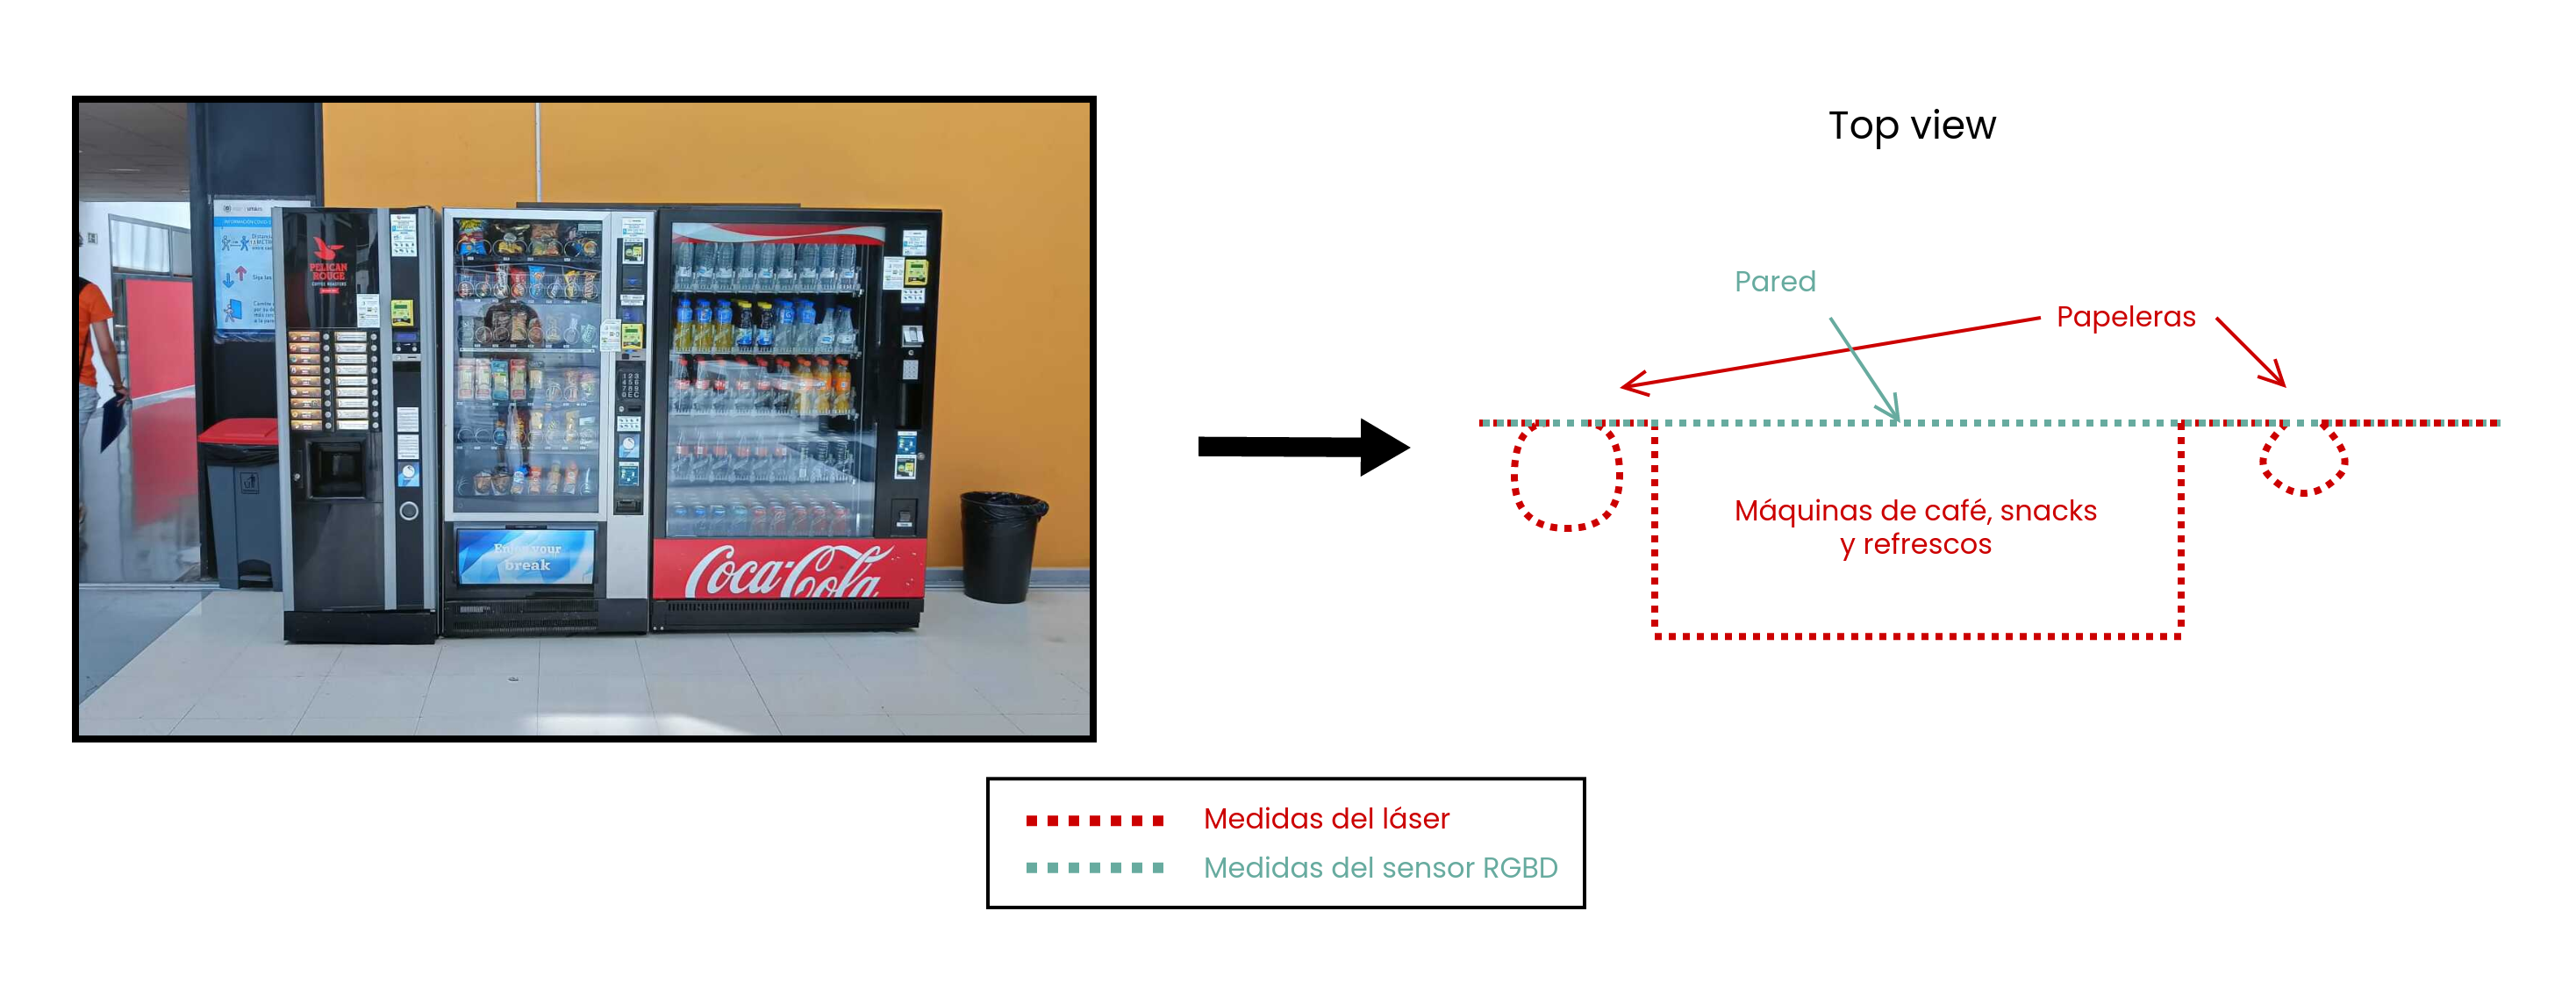
\includegraphics[width=\textwidth]{laser_vs_rgbd.png}
	\end{center}
	\caption{Comparación teórica del resultado de una medición de un láser 2D y un sensor RGBD sobre elementos presentes en la Escuela de Ingenierías Industriales.}
	\label{fig:laser_vs_rgbd}
\end{figure}

En este proyecto se pretende analizar una posible solución al problema de fiabilidad en la representación de los mapas de ocupación realizados con sensores LIDAR mediante el uso de sensores RGBD para generar \textit{floorplans} fieles a la estructura invariable del entorno. Entre las utilidades de conseguir un mapa sin los objetos móviles, las más destacadas son:

\begin{itemize}

	\item La más importante es la posibilidad de tener un mapa que permita al robot localizarse aún con los cambios que puedan surgir a lo largo del tiempo en los elementos que conforman el entorno. Así se evita tener que generar un nuevo mapa cada vez que surja algún cambio significativo.
	\item En aplicaciones de realidad aumentada para el diseño de interiores, este sistema permitiría obtener las dimensiones reales de la vivienda y así tener una idea en primera persona del cambio de mobiliario o de una nueva organización del mismo.
	\item Normalmente existe una clara disparidad entre el plano de una vivienda o de un edificio diseñado por el arquitecto y el producto final. Con este mapa generado sería posible comparar y obtener un plano fiel a la realidad y así validar las dimensiones reales de la infraestructura.

\end{itemize}



\section{Objetivo}

Dado que los robots utilizan los mapas de ocupación o \textit{floorplans} para localizarse y navegar en un entorno, es necesario que éstos sean lo más fiel posible a la estructura real del edificio o de la vivienda. Esto resulta imposible si durante la fase de obtención del mapa existen elementos que no pertenecen a la infraestructura, ya que provocan que el mapa resultante no sea fiel a las dimensiones reales del entorno.\\

Debido a la necesidad y utilidad de obtener mapas de ocupación sin elementos cambiantes, el objetivo de este trabajo es utilizar la información proporcionada por sensores RGBD para la generación de \textit{floorplans}, solucionando problemas de variabilidad en el entorno que perjudican seriamente la fiabilidad del mapeado mediante sensores láser.\\

Se obtendrá información acerca de la profundidad de los píxeles captados y se escogerán aquellos puntos menos restrictivos (más alejados) para generar un láser artificial que permita la creación del mapa de ocupación mediante algoritmos de mapeado.\\

Paralelamente, se utilizará un modelo entrenado de inteligencia artifical, YOLO, para detectar los elementos de la imagen de color y así llevar un registro de los objetos que se ha encontrado el robot en su trayectoria.\\

Finalmente, se hará una comparativa de los resultados obtenidos únicamente con el LIDAR con los obtenidos mediante el procesamiento de la información de la cámara. Además se hará un estudio de los objetos detectados durante el mapeado y de la fiabilidad del modelo de detección. \\

\section{Estructura del documento}

Este documento está dividido en cuatro partes. En la primera parte se hará una introducción al contexto del proyecto y se explicará por qué se ha desarrollado.\\

La segunda parte consta de tres capítulos. En el primero de ellos se expondrán las herramientas utilizadas y se explicarán brevemente cómo se utilizan y porqué se han escogido. En un segundo capítulo, el más importante, se desarrollará el trabajo y se explicará cómo se ha llevado a cabo. En el tercer y último capítulo se expondrán los resultados y se compararán con los ideales, comentando sus diferencias y problemas encontrados.\\

En la tercera parte se mostrarán las conclusiones obtenidas tras la consecución del proyecto y se comentarán algunas posibles líneas de trabajo abiertas de cara al futuro, así como posibles mejorías que se pudieran implementar. \\

En una cuarta y última parte se sitúan los apéndices del proyecto. En el primero se explica el software que se ha utilizado de apoyo pero que no se ha mencionado en los capítulos anteriores. En el segundo apéndice se expone el código de los nodos que han sido diseñados expresamente para este trabajo.\\



























